% Template for ICIP-2013 paper; to be used with:
%          spconf.sty  - ICASSP/ICIP LaTeX style file, and
%          IEEEbib.bst - IEEE bibliography style file.
% --------------------------------------------------------------------------
\documentclass{article}
%\usepackage{spconf,amsmath,graphicx,hyperref,ulem}
%\usepackage{spconf,amsmath,graphicx,hyperref}
\usepackage{spconf,amsmath,graphicx,color,amsfonts,algorithm,algpseudocode,epsfig,subfigure}

% Example definitions.
% --------------------
\def\x{{\mathbf x}}
\def\L{{\cal L}}

% Title.
% ------
\title{Occlusion Invariant Face Hallucination}
%
% Single address.
% ---------------
\name{Shun-Jen Lee$^{1,2}$, Meng-Huan Wu$^{1,2}$, Chia-Po Wei$^2$, Yu-Chiang Frank Wang$^2$}
\address{$^1$Department of Electrical Engineering, National Taiwan University, Taipei, Taiwan\\
$^2$Research Center for IT Innovation, Academia Sinica, Taipei, Taiwan}
%
% For example:
% ------------
%\address{School\\
%	Department\\
%	Address}
%
% Two addresses (uncomment and modify for two-address case).
% ----------------------------------------------------------
%\twoauthors
%  {A. Author-one, B. Author-two\sthanks{Thanks to XYZ agency for funding.}}
%	{School A-B\\
%	Department A-B\\
%	Address A-B}
%  {C. Author-three, D. Author-four\sthanks{The fourth author performed the work
%	while at ...}}
%	{School C-D\\
%	Department C-D\\
%	Address C-D}
%

\newcommand{\ub}{\mathbf{u}}
\newcommand{\xb}{\mathbf{x}}
\newcommand{\Ib}{\mathbf{I}}

\newcommand{\topcaption}{%
  \setlength{\abovecaptionskip}{-20pt}%
  \setlength{\belowcaptionskip}{0pt}%
  \caption}
\begin{document}
%\ninept
%
\maketitle
%
\begin{abstract}
Face images captured by surveillance cameras are generally noisy and with low resolution (LR). In addition, such images might be corrupted due to occlusion or disguise, which would make the recovery of their high resolution (HR) versions very challenging. In this paper, we propose a face hallucination method which is robust to occlusion or undesirable artifacts. Based on sparse representation, our method is able to identify the corrupted image pixels without any prior knowledge on the type of occlusion for the LR inputs, while the pixels of interest for the HR outputs will be synthesized by solving sparse coding tasks. Experimental results confirm that our approach not only results in satisfactory image quality for the recovered HR outputs, improved recognition performance will also be achieved for LR-to-HR recognition tasks.

%Matching individuals across non-overlapping camera views is known as the problem of person re-identification. In addition to significant visual appearance variations due to lighting, view angle, etc. changes, one might encounter corrupted data due to background clutter and occlusion, or even missing data at some camera views in practical scenarios. To address the above challenges, we present a novel approach to robust person re-identification, particularly aiming at handling missing and corrupted image data across camera views. Based on the technique of low-rank matrix decomposition, our proposed algorithm observes the low-rank structure of cross-view data, which is able to disregard extreme/sparse errors while the missing instances can be recovered automatically. Our experiments will confirm the effectiveness and robustness of our method, which is shown to outperform several baseline and state-of-the-art person re-identification approaches.


%Instead of relying on prevailing linearization, coarse-to-fine warping, and descriptor-based matching techniques to estimate large motion on two consecutive frames,  we use gradient descend to jointly minimize both data term and smoothness term in the proposed energy function at superpixel-level. We found that optimizing data term could be treated as doing the mean-shift tracking on all superpixels simultaneously. Moreover, by using anisotropic nonlocal smoothness term which passes matching information within the same object, we greatly alleviates local minimum problem which troubles many other optical flow algorithms. Finally, an promising experiment results demonstrate our method as an effective new type of way to solve large displacement optical flow problem.
\end{abstract}
%
\begin{keywords}
Face Hallucination, Face Recognition, Sparse Representation
\end{keywords}
%

\section{Introduction}
\input{introduction.tex}

\section{Our Proposed Method}
%\subsection{Robust Sparse Coding}
%\label{subsec:RSC}
%
%\label{subsec:RSC}

\newcommand{\bW}{\mathbf{W}}
\newcommand{\by}{\mathbf{y}}
\newcommand{\bx}{\mathbf{x}}
\newcommand{\bD}{\mathbf{D}}
\newcommand{\norm}[1]{\left\|#1 \right\|}
\newcommand{\Real}{\mathbb{R}}
\newcommand{\balpha}{\boldsymbol{\alpha}}

{
Since the LR input images may be partially occluded, we need to detect the occluded region in advance before further processing. In this work, we utilize robust sparse coding (RSC) \cite{Yang_CVPR2011} to handle occlusion.
Let $\by_L\in\Real^d$ be the LR test image and $\bD_L\in\Real^{d\times n}$ be the LR training dictionary, i.e., $\bD_L = [\bx_{L,1},\bx_{L,2},\cdots,\bx_{L,n}]$, where $\bx_{L,i}\in\Real^d$ is the $i$th LR training image. The algorithm of RSC repeated solving a weighted sparse coding problem and updating a weight matrix. The formulation of the weighted sparse coding problem is as follows:
\begin{equation} \label{eq:RSCProblem}
\min_{\balpha_L}\norm{\bW_L(\by_L-\bD_L\balpha_L)}_2^2+\lambda\norm{\balpha_L}_1,
\end{equation}
where the weight matrix $\bW_L$ is given by
\begin{equation} \label{eq:W}
\bW_L = \mbox{diag}(w(e_{1}), w(e_{2}), \ldots, w(e_{d}))^{1/2},
\end{equation}
\begin{equation}\label{eq:weight}
w(e_{k}) = \frac{exp(-\mu e_{k}^{2}+\mu\delta)}{1+exp(-\mu e_{k}^{2}+\mu\delta)},
\end{equation}
where $e_k$ is the $k$th entry of $\mathbf{e} = \by_L-\bD_L\balpha_L$. The weight function $w(e_{k})$ outputs a small value when the magnitude of $e_k$ is large. As a result, RSC can lower the influence of poorly reconstructed pixels. In \eqref{eq:weight}, the product $\mu\delta$ is chosen to be a large constant, and $\delta$ is the $j$th largest entry in the vector $[e_{1}^{2},e_{2}^{2}\ldots e_{d}^{2}]$. RSC choose $j$ as the nearest integer to $\tau d$ with $\tau \in [0.6, 0.8]$. Note that when $\bW_L$ is fixed, \eqref{eq:RSCProblem} becomes a standard L1-minimization problem. In all of our experiments, we utilize the Homotopy method for solving \eqref{eq:RSCProblem} because of its efficiency as suggested in \cite{L1review}.
} 


\subsection{Occlusion Invariant Sparse Coding}
\label{subsec:aRSC}
\newcommand{\bW}{\mathbf{W}}
\newcommand{\by}{\mathbf{y}}
\newcommand{\bx}{\mathbf{x}}
\newcommand{\be}{\mathbf{e}}
\newcommand{\bD}{\mathbf{D}}
\newcommand{\te}{\tilde{\mathbf{e}}}
\newcommand{\balpha}{\boldsymbol{\alpha}}
\newcommand{\btau}{\boldsymbol{\tau}}
\newcommand{\bPhi}{\boldsymbol{\Phi}}
\newcommand{\norm}[1]{\left\|#1 \right\|}
\newcommand{\Real}{\mathbb{R}}
\newcommand{\bemx}{\begin{bmatrix}}
\newcommand{\enmx}{\end{bmatrix}}

For practical face hallucination scenarios, the input LR images might be corrupted due to occlusion or disguise, and thus it would be crucial to develop a hallucination algorithm which is robust to such undesirable effects. In our work, we propose a sparse representation based algorithm to recover the image regions of interest in the HR outputs, while the corrupted ones will be simplified predicted by interpolation based techniques (and be disregarded if recognition is performed).

Before detailing our proposed method, we first define the notations and variables for the sake of clarification. Let $\by_L\in\Real^d$ be the LR input image, which might be partially occluded. We have $\bD_L\in\Real^{d\times n}$ as the LR training dictionary of $n$ instances, i.e., $\bD_L = [\bx_{L,1},\bx_{L,2},\cdots,\bx_{L,N}]$, where $\bx_{L,i}\in\Real^d$ denotes the $i$th LR training image and $N$ is the number of training images. To solve image representation problems with occlusion, Yang \emph{et al.}~\cite{Yang_CVPR2011} recently presented robust sparse coding (RSC), which represents the LR input by solving

\begin{equation} \label{eq:RSCProblem}
\min_{\balpha_L}\norm{\bW_L(\by_L-\bD_L\balpha_L)}_2^2+\lambda\norm{\balpha_L}_1,
\end{equation}
where the weight matrix $\bW_L$ is defined as
\begin{equation}\label{eq:weight}
\begin{split}
&\bW_L = \mbox{diag}(w(e_{1}), w(e_{2}), \ldots, w(e_{d}))^{1/2},\\
&\mbox{and}~~w(e_{k}) = \frac{exp(-\mu e_{k}^{2}+\mu\delta)}{1+exp(-\mu e_{k}^{2}+\mu\delta)}.
\end{split}
\end{equation}
In~\eqref{eq:weight}, $e_k$ indicates the $k$th entry of $\mathbf{e} = \by_L-\bD_L\balpha_L$, which represents the reconstruction error for the $k$th image pixel in the LR input. The function $w(e_{k})$ is designed to produce a small value when the magnitude of $e_k$ is large (and vice versa). In~\cite{Yang_CVPR2011}, the product $\mu\delta$ is chosen to be a large constant, and $\delta$ is the $j$th largest entry in the vector $[e_{1}^{2},e_{2}^{2}\ldots e_{d}^{2}]$. RSC has $j$ as the nearest integer to $\tau d$ with $\tau \in [0.6, 0.8]$. Nevertheless, the goal of RSC is to suppress the influence of poorly reconstructed pixels.

%Note that when $\bW_L$ is fixed, \eqref{eq:RSCProblem} becomes a standard L1-minimization problem. In all of our experiments, we utilize the Homotopy method for solving \eqref{eq:RSCProblem} because of its efficiency as suggested in \cite{L1review}.

It is worth noting that $\tau$ can be interpreted as the proportion of non-occluded image pixels to the total pixel number in the LR input. For example, if we set $\tau$ as 0.6, 40\% percent of pixels associated with the largest (poorest) reconstruction errors will be suppressed. In other words, the remaining 60\% of the pixels will be recovered by $\bD_L$. Unfortunately, there is no guideline in~\cite{Yang_CVPR2011} to determine this crucial parameter $\tau$, and thus it might not be easy to apply RSC for practical scenarios.

To overcome the above problem, we propose a maximum likelihood estimation (MLE)~\cite{Bishop_2006} based approach for determine the optimal $\tau$, which allows us to recover the non-occluded image regions with performance guarantees. Instead of setting $\tau$ as a fixed value for all input images, we first observe the recovered images with varying $\tau$ values. Figure~\ref{fig_regression} shows an example, in which each point denotes the total reconstruction error for non-occluded image pixels with a particular $\tau$ value. More specifically, by varying the value of $\tau$, we obtain a set of points $(\tau_1,e_1), \ldots, (\tau_M,e_M)$.

% fig: idealCurve
\begin{figure}[!t]
\graphicspath{{fig/}}
        \begin{center}
            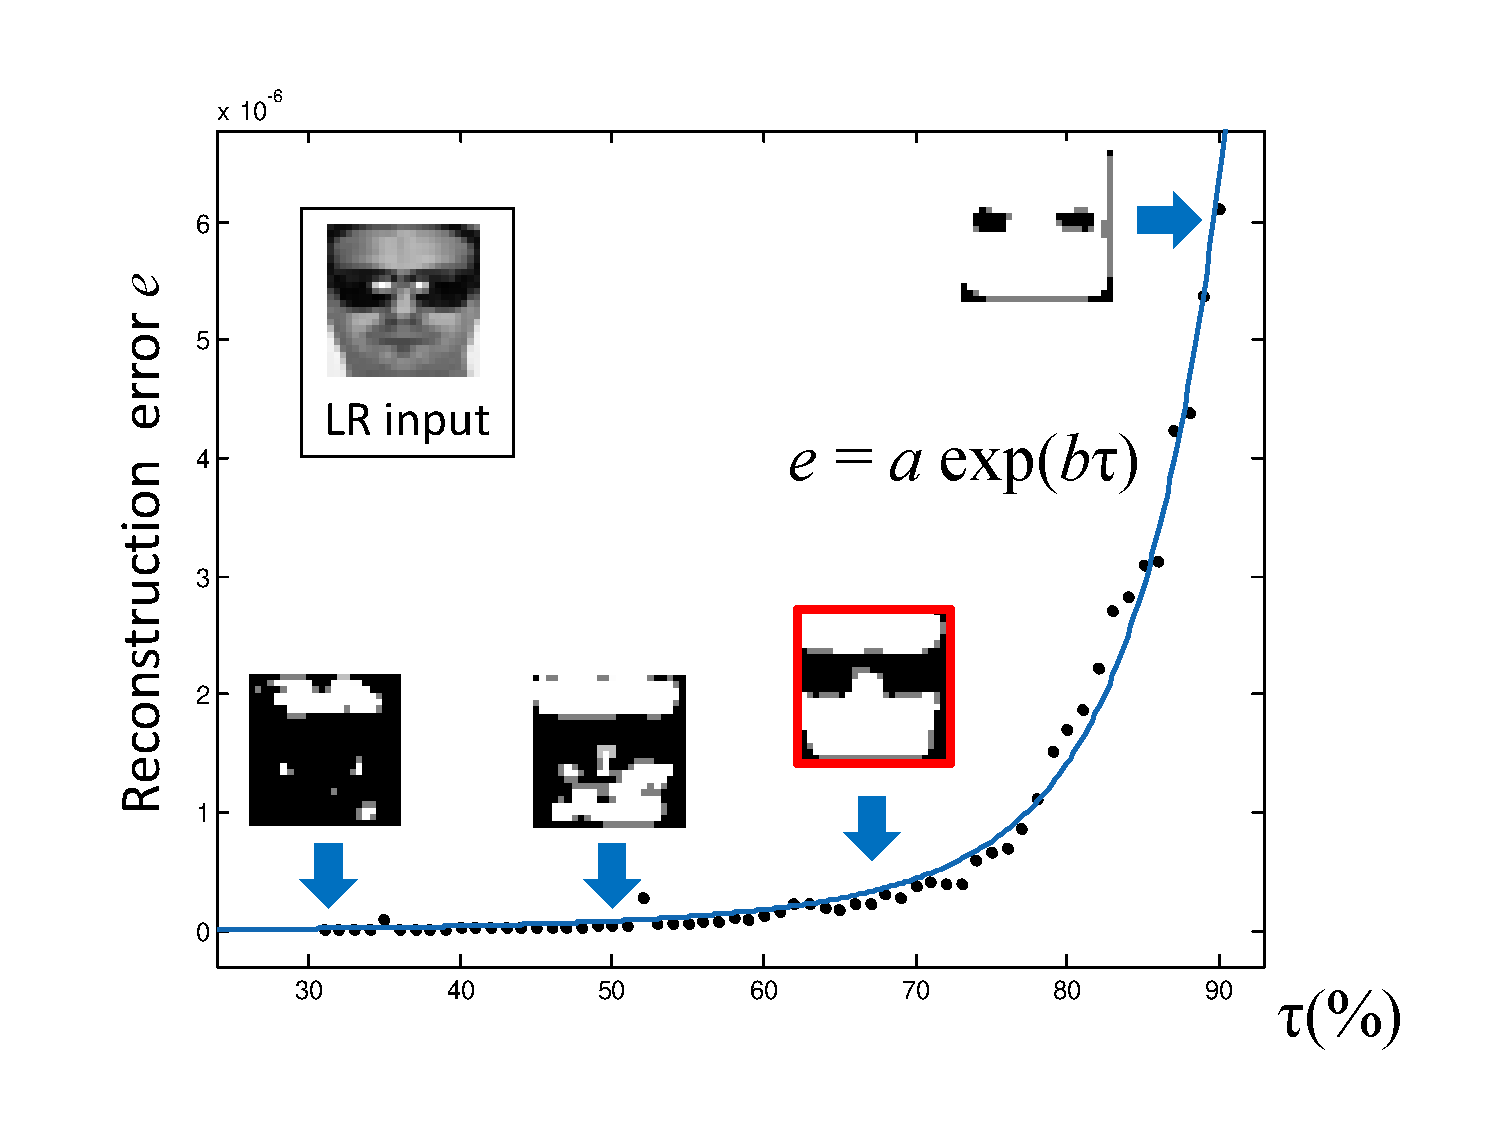
\includegraphics[scale=0.30]{exponential_regression.pdf}
            \vspace{-0.2cm}
            \caption{\small{Reconstruction errors of non-occluded image regions with varying $\tau$ values. The blue curve is an exponential function $e=a\exp(b\tau)$ fitting the observed instances. Note the the preferable recovered image is bounded by a red rectangle.}}\label{fig_regression}\vspace{-.5cm}
        \end{center}
\end{figure}

In order to determine the optimal $\tau$ for obtaining the preferable recovered face image (i.e., the one with red rectangle in Figure~\ref{fig_regression}), we need to first fit the observed points with an exponential function, i.e.,
\begin{equation}\label{eqn_exponential}
     e = f(\tau,a,b) = a\exp(b\tau),
\end{equation}
where $a$ and $b$ are the parameters to be determined. Note that $f(\tau,a,b)$ in \eqref{eqn_exponential} is a nonlinear function of $\tau$. To make the fitting problem more tractable, we take the logarithm of both sides of~\eqref{eqn_exponential} and obtain $\ln (e) = \ln (a) + b\tau$. Based on MLE, we approach this curve fitting task by solving the following optimization problem:
\begin{equation}\label{eqn_ls}
    \min_{a,b}\sum_{m=1}^M \left(\ln(e_m)-\ln(a)-b\tau_m\right)^2.
\end{equation}
By defining $\tilde{a} = \ln(a)$, the above minimization problem can be expressed as
\begin{equation}\label{eqn_ls_eq}
    \min_{\tilde{a},b} \norm{\te-[\mathbf{1}, \btau]\bemx \tilde{a}\\ b\enmx}_2^2,
\end{equation}
where $\te = [\ln(e_1),\ldots,\ln(e_M)]^T$, $\btau = [\tau_1,\ldots,\tau_M]^T$, and $\mathbf{1} = [1,\ldots,1]^T\in\Real^M$. We note that~\eqref{eqn_ls_eq} is a standard least squares problem, and its analytical solution is dervied by
\begin{equation}\label{eqn_ls_sol}
     \bemx \tilde{a}\\b \enmx = (\bPhi^T\bPhi)^{-1}\bPhi^T\te
\end{equation}
with $\bPhi := [\mathbf{1}, \btau]$. Once we have $\tilde{a}$, the parameter $a$ is obtained as $a = \exp(\tilde{a})$.

With parameters $a$ and $b$ for the exponential curve~\eqref{eqn_exponential} learned by MLE, we now discuss how to determine the optimal $\tau$ for recovering the image without occluded pixels (e.g., the one bounded by the red rectangle in Figure~\ref{fig_regression}). In our work, we empirically observe that the optimal $\tau$ always corresponds to the intersection of the reconstruction curve and the straight line with a fixed slope $s$ as shown in Figure~\ref{fig_slopes}. Moreover, this slope $s$ does \emph{not} vary with different types of face images (occluded or not).

In our work, the value of $s$ can be directly observed from training data, which is a constant over images with different degrees of occlusion (as illustrated in Figure~\ref{fig_slopes}). Once the value of $s$ is known, we can begin to calculate parameter $\tau$. To solve this task, we set the derivative of~\eqref{eqn_exponential} with respect to $\tau$ equal to $s$. As a result, we have $\frac{de}{d\tau} = ab\exp(b\tau) = s$, and the optimal $\tau$ is obtained as follows
\begin{equation}\label{eqn_tau}
     \tau = \frac{1}{b}(\ln(s)-\ln(ab)).
\end{equation}
Different from RSC which requires one to manually select $\tau$ for representing the input image, our method is able to automatically select the best $\tau$ for each input without any prior knowledge on the type of occlusion, which is preferable for practical hallucination tasks. Thus, we refer to this proposed encoding process as \emph{occlusion invariant sparse coding}.

Once the optimal $\tau$, we apply~\eqref{eq:weight} for calculating the associated weight matrix $\bW_L$. For refinement purposes, a median filter is applied to the resulting $\bW_L$ which preserves the completeness and smoothness of the determined occluded regions.




\begin{figure}
\graphicspath{{fig/}}
    \begin{center}
        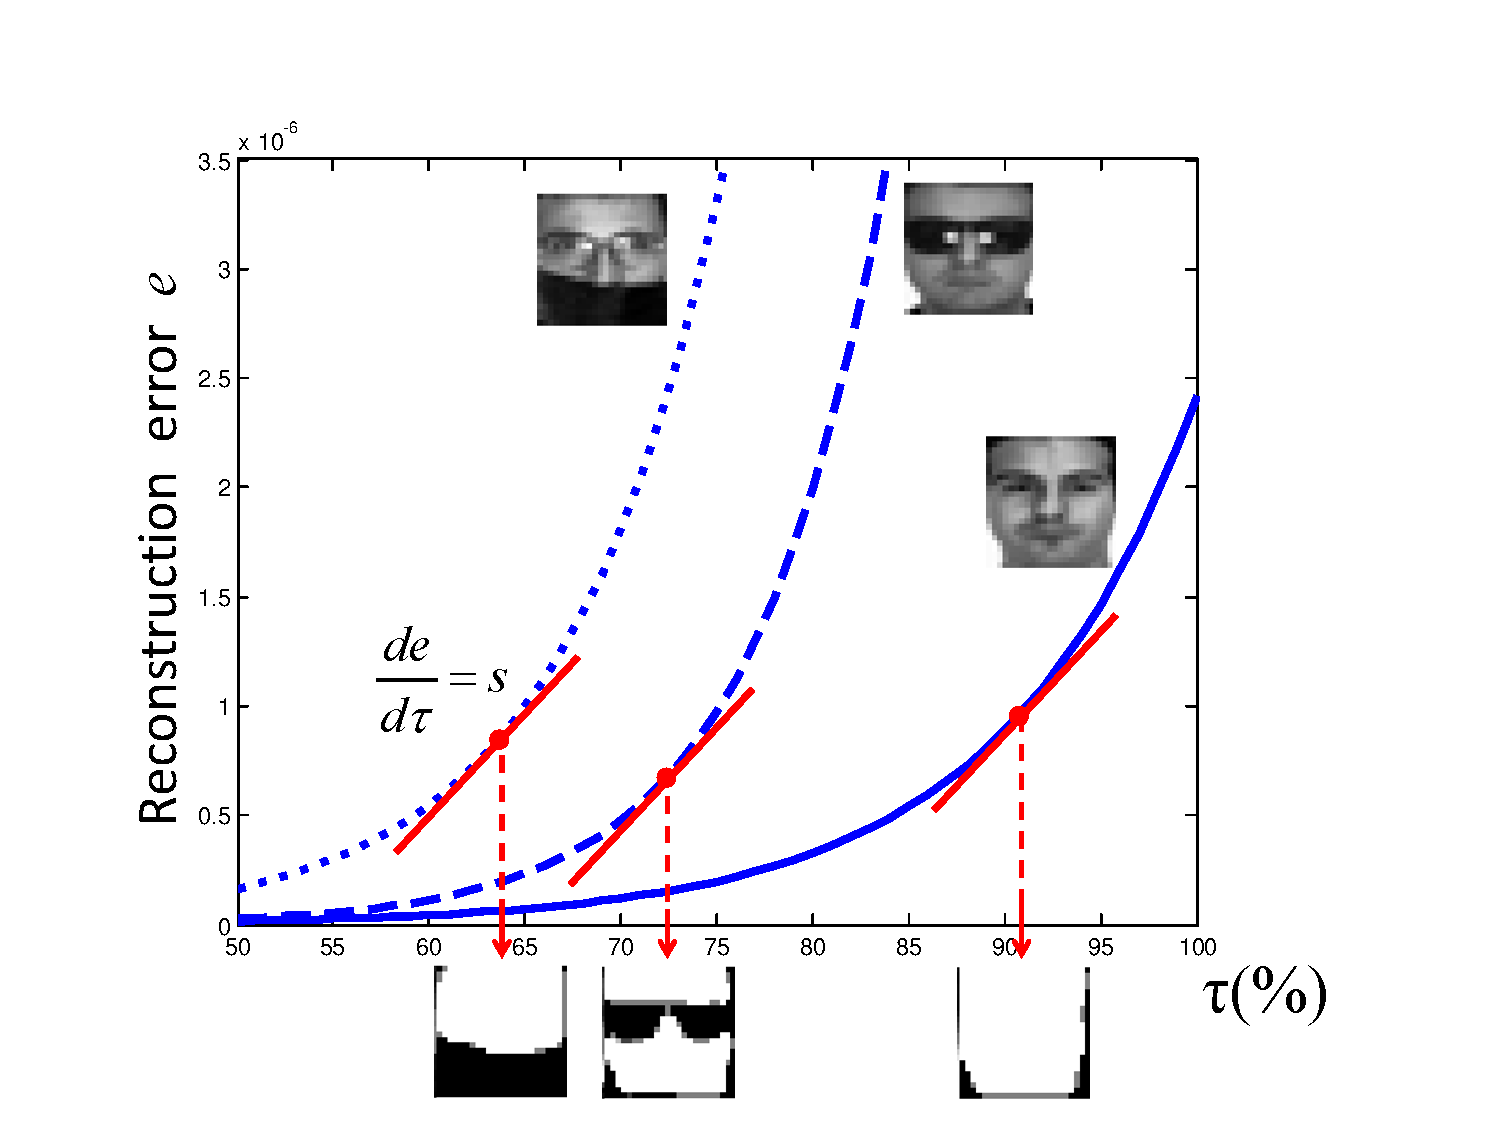
\includegraphics[scale=0.32]{ARSC_slopes.pdf}
        \vspace{-0.2cm}
        \caption{\small{Fitting curves of reconstruction errors $e$ vs. $\tau$ for three face images with different degrees of occlusion. The points of tangency depict the optimal $\tau$ for recovering non-occluded image regions.}}\label{fig_slopes}
        %\topcaption{The appropriate slope for determining $\tau$. Although the two input images (i.e., the occluded one and the neutral one) have different proportion of occluded pixels, this pre-defined slope can identify the occluded region nicely.\label{fig:cutSlope}}
    \end{center}\vspace{-.5cm}
\end{figure}


\subsection{Occlusion Invariant Sparse Representation for Face Hallucination}
\label{subsec:hallucination}
{

%fig5 : is separated, back in experiment.tex
\iffalse
\begin{figure*}[!Htbp]

\graphicspath{{fig/}}
    \centering
        \subfigure{ 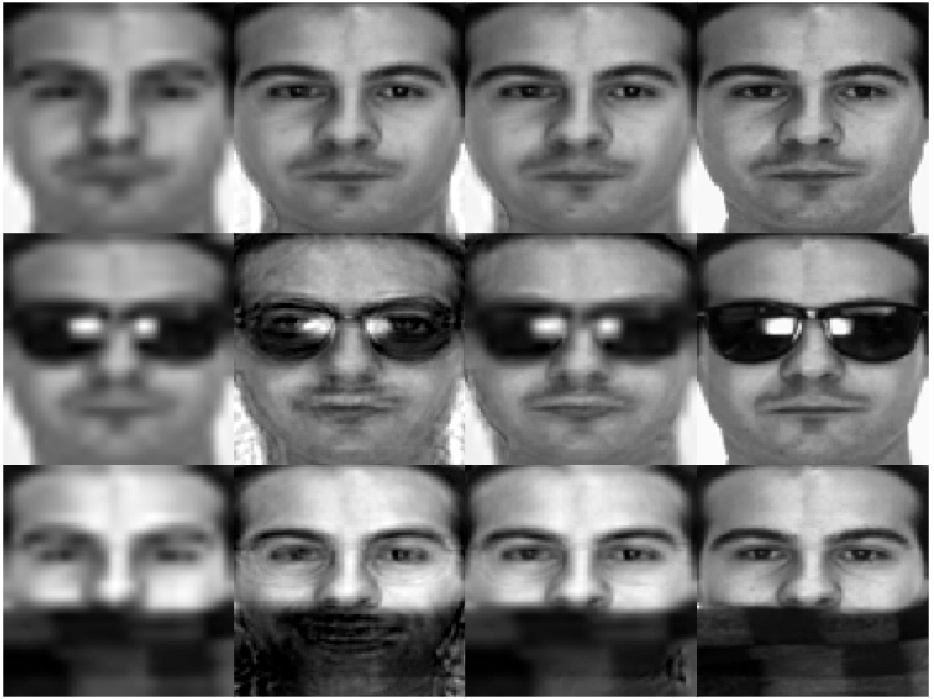
\includegraphics[scale=0.25]{exp_ori.jpg}}
        \subfigure{ 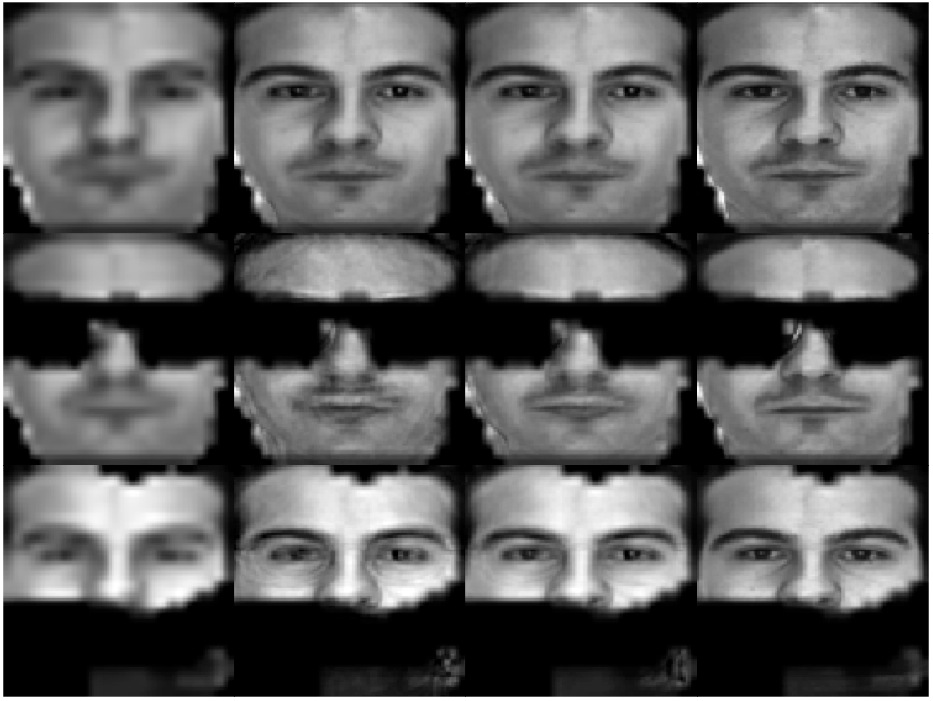
\includegraphics[scale=0.25]{exp_masked.jpg}}
    \caption{The hallucination result of experiment. The columns in each side are (a) Bicubic (b) Jung's Method \cite{convex}, (c) our proposed method, and (d) ground truth respectively\label{fig:exp}}
\end{figure*}
\fi

With the proposed occlusion invariant sparse coding scheme in Section~\ref{subsec:aRSC}, we are able to derive the sparse coefficients for representing the LR input $\by_L$ using LR dictionary $\bD_L$. To predict the corresponding HR output image, we apply the sparse representation based super resolution techniques of~\cite{TIP10,convex} for our face hallucination task, as we now discuss.

Given the LR dictionary and its corresponding HR version $\bD_H\in\Real^{m\times n}$, it is assumed in~\cite{TIP10,convex} that the sparse coefficients for representing the HR image $\by_H\in\Real^m$ would be identical to those for its LR input $\by_L\in\Real^d$. However, since approaches like~\cite{TIP10,convex} are not robust to occluded regions, we need to apply the proposed occlusion invariant sparse coding scheme for addressing this challenging problem.

Recall that, in Section~\ref{subsec:aRSC}, our proposed algorithm is able to derive the weighting matrix $\bW_L$ from $\by_L$ and $\bD_L$, which indicates and recovers the non-occluded image regions while suppressing corrupted pixels. For hallucinating the HR image, we first extend the derived matrix $\bW_L$ to $\bW_L\in\Real^{m\times m}$ via interpolation. Next, we consider patch-based sparse representation for performing occlusion invariant face hallucination. That is, we divide the LR input $\by_L$ into overlapping patches, denoted by $\by_L^i$, where $i$ is the patch index. Similary, each LR training image in $\bD_L$ is also divided into overlapping patches, denoted by $\bx_{L,j}^i$ for $j=1, 2,~\ldots, N$. 

Now, the sparse coefficient for the $i$th patch can be determined by solving the following problem:
\begin{equation}\label{eqn1}
     \min_{\balpha_L^i} \norm{\bW_L^i(\by_L^i - \bD_L^i\balpha_L^i)}_2^2+\lambda\norm{\balpha_L^i}_1,
\end{equation}
where $\bW_L^i$ indicates the $i$th patch of $\bW_L$. With $\balpha_L^i$ calculated, the $i$th output patch can be derived~by
\begin{equation}
\by_H^i = \bW_H^i\bD_H^i\balpha_L^i,
\end{equation}
where $\bW_H^i$ is the $i$th patch in $\bW_H$, and $\bD_H^i$ indicates the $i$th patches of $\bD_H$. Once all the patches for the HR output is obtained, hallucination of $\by_H$ is complete. We note that, for occluded image regions in $\by_H$, we simply perform bicubic interpolation on the associated regions of the LR input. The framework of our method is depicted in Figure~\ref{fig:algFlow}.

}


%\mathop{\arg\min}_\limits{w_{m}(i,j)}



\section{Experiments}
\label{sec:exp}
\subsection{Database and Settings}
We consider the AR database~\cite{Martinez_CVC1998} for evaluation, which contains 126 individuals with more than 4000 frontal face images. In our experiment, we consider a subset of AR by randomly choosing 100 individuals with 50 men and 50 women. All images are converted into grayscale. We crop and rescale the images into 96$\times$96 and 24$\times$24 pixels as HR and LR images, respectively. For each subject in AR, we only consider the neutral image and images with expression variations from Session 1 in the training set. The remaining ones in both sessions are viewed as test images.
%figure 5
\begin{figure}
\graphicspath{{fig/}}
        \begin{center}
            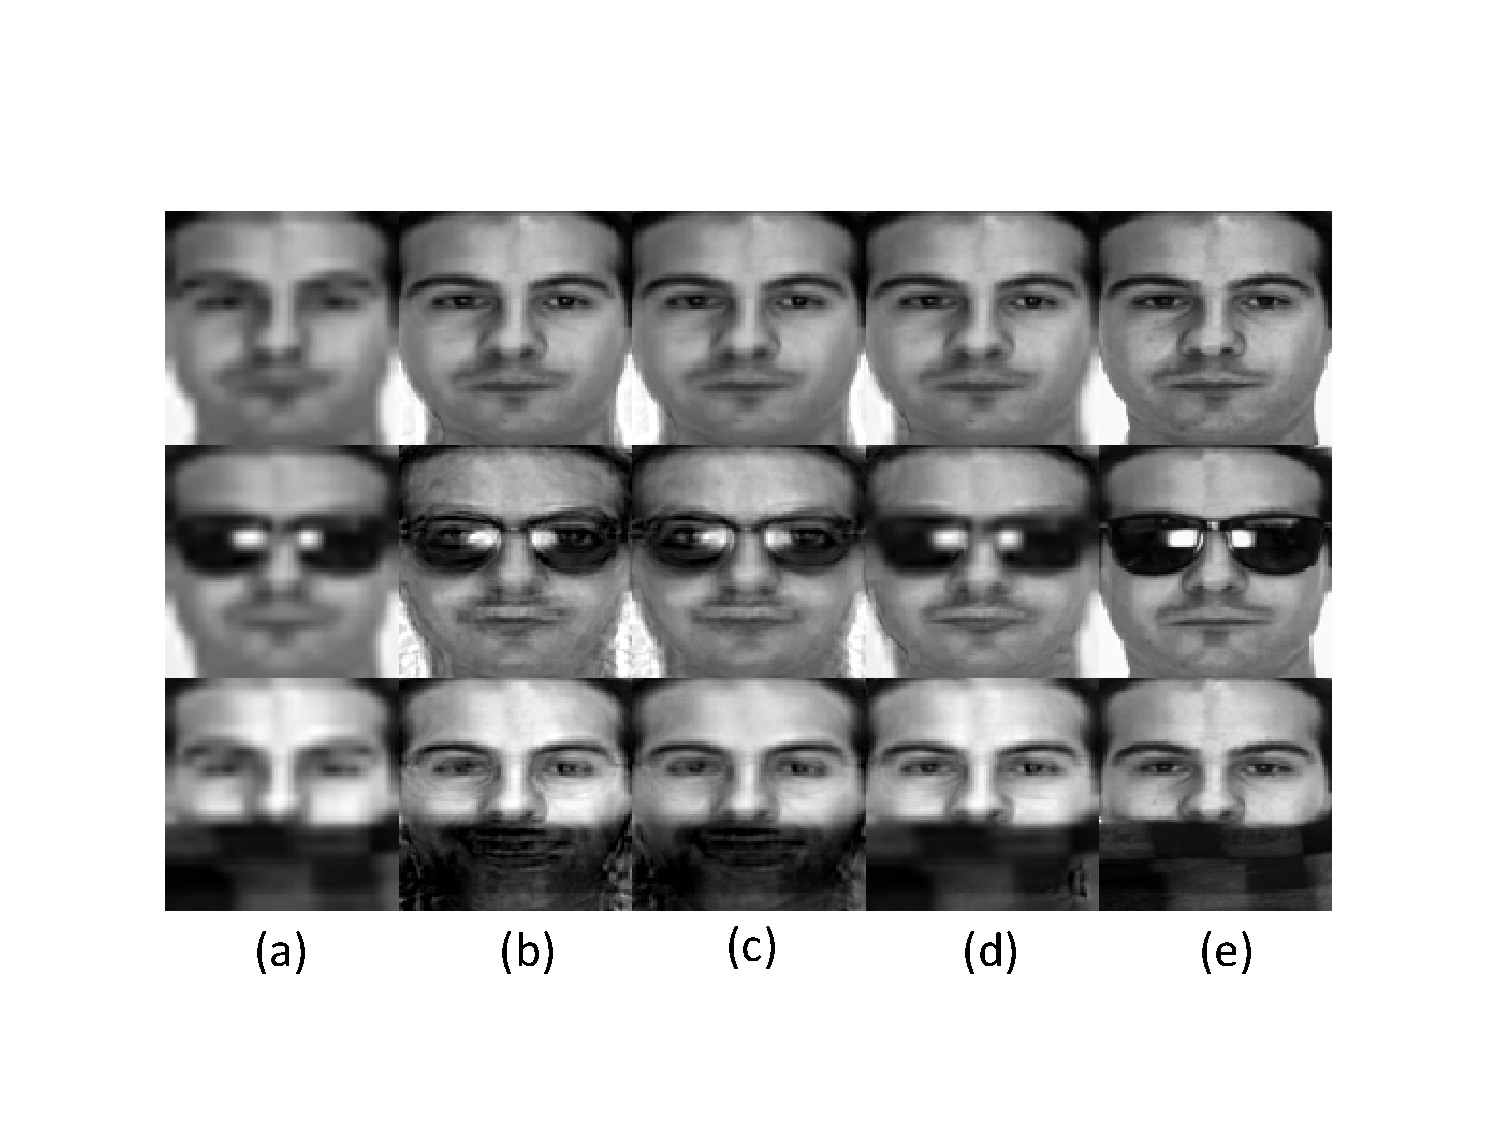
\includegraphics[scale=0.32]{exp_ori.pdf}
            \vspace{-0.3cm}
            \caption{\small{Example face hallucination results including occluded image regions. Images in each row are outputs of (a) Bicubic, (b) Jung \emph{et al.}~\cite{convex}, (c) Jiang \emph{et al.}~\cite{Jiang_TMM2014}, (d) ours, and (e) the ground truth.} \label{fig:exp_ori}}
        \end{center}\vspace{-.5cm}
\end{figure}

% table1
\begin{table}
\small
\renewcommand{\arraystretch}{1.2}
\centering
\caption{\small{Comparisons of average PSNR \& SSIM values of face hallucination outputs with occlusion.}}\label{tab:partA}
\vspace{0.2cm}
\begin{tabular}{|c|c|c|c|c|}
\hline
 & Bicubic & \cite{convex} & \cite{Jiang_TMM2014}  & Ours\\
\hline
PSNR  & 24.09 & 23.67 & 24.05 & \textbf{24.58}\\
\hline
SSIM  & 0.7975 & 0.7240 & 0.7404 & \textbf{0.8094}\\
\hline
\end{tabular}\vspace{-.3cm}
\end{table}

\subsection{Face Hallucination}

To evaluate our face hallucination results, we consider the LR face image inputs with and without occlusion. In addition, since our method is able to identify the corrupted pixels automatically, we further include the evaluation of recovered HR images using non-occluded pixels only. This is to show that, after disregarding such undesirable pixels, our method is able to achieve improved image quality for face hallucination.

We first compare the example outputs in Figure~\ref{fig:exp_ori}, in which the HR images (including the occluded image regions) are produced by bicubic, the approaches of \cite{convex} and \cite{Jiang_TMM2014}, and ours. In addition, we also show the ground truth HR images in the last column of Figure~\ref{fig:exp_ori}. From this figure, we see that our approach achieved satisfactory image quality for non-occluded image regions. Recall that our method views occluded regions as image corruption, and thus the corresponding pixels are produced by bicubic interpolation. In Table~\ref{tab:partA}, we quantitatively compare the image quality using PSNR and SSIM values. It can be seen that our approach was able to achieve improved results than other SR methods did.

Next, we consider the comparisons in which the HR images are corruption free. In other words, we apply our proposed method to remove the undesirable image pixels (mainly due to occlusion) from the HR images of different approaches. Figure~\ref{fig:exp_msk} and Table~\ref{tab:partB} present and compare the results of different approaches. We see that, after removing such corrupted image pixels, our method still obtained improved image quality for the remaining pixels of interest, and thus performed favorably against other SR approaches. Therefore, from the above qualitative and quantitative evaluation, the effectiveness of our proposed method for occlusion invariant face hallucination can be successfully verified.

%figure 6
\begin{figure}
\graphicspath{{fig/}}
        \begin{center}
            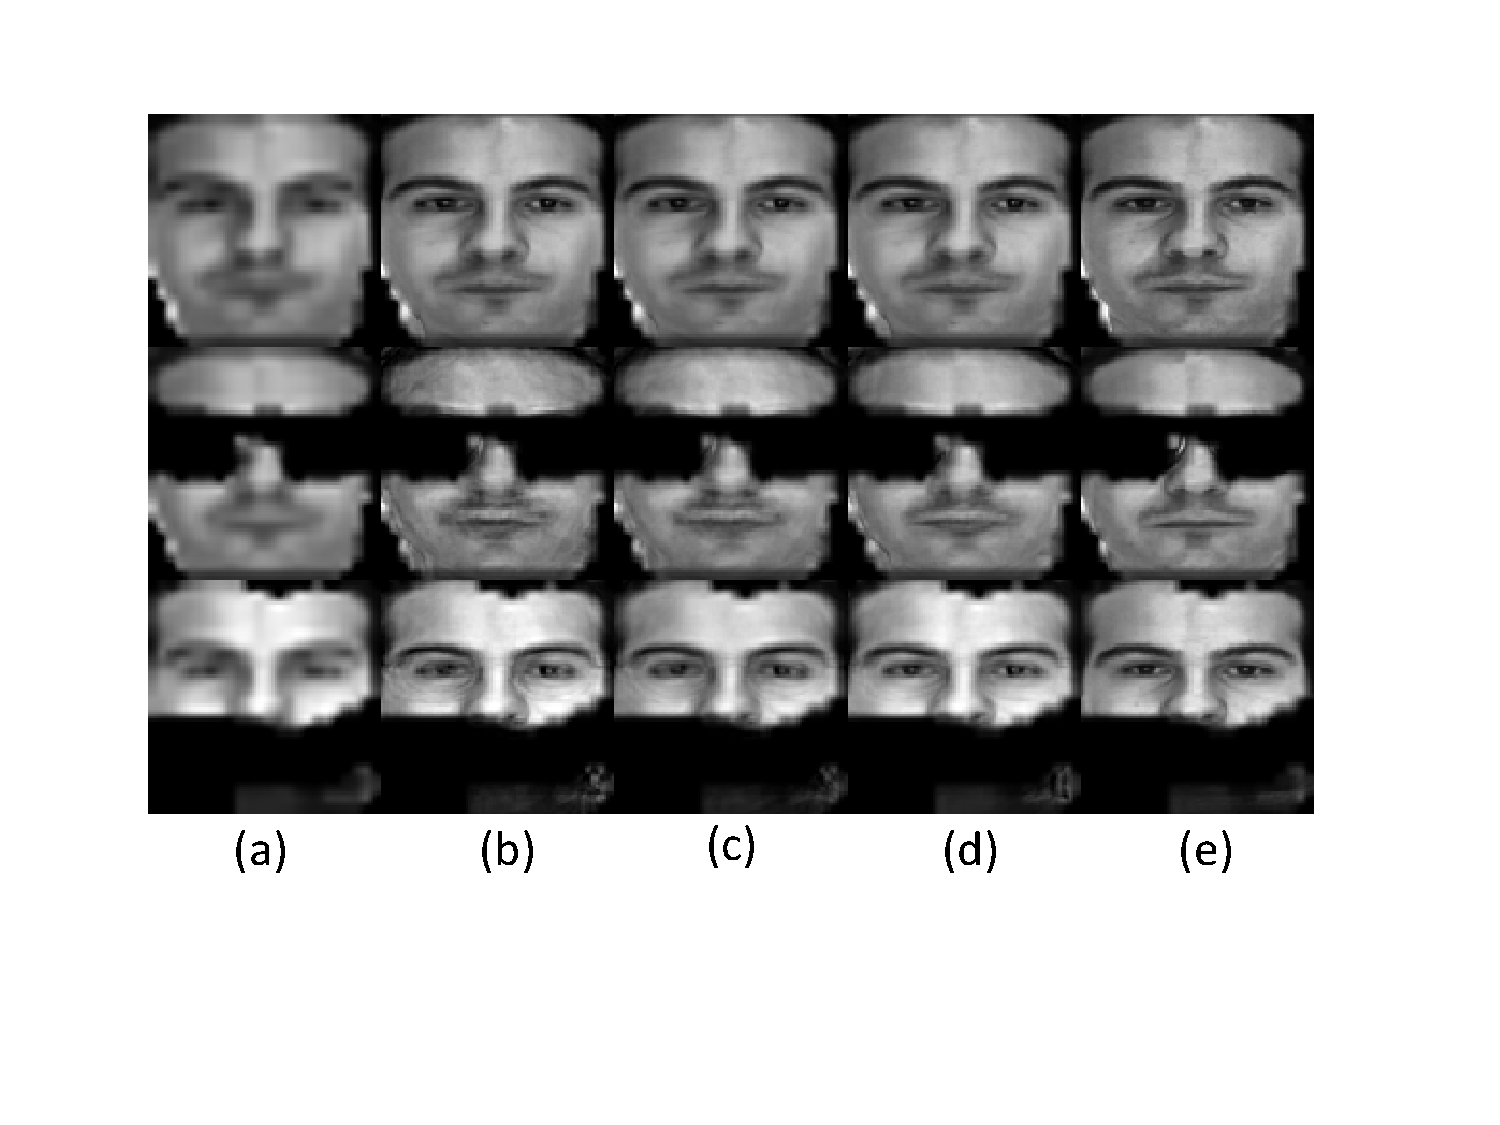
\includegraphics[scale=0.32]{exp_masked.pdf}
            \vspace{-0.3cm}
            \caption{\small{Example face hallucination results with corrupted pixels removed. Images in each row are outputs of (a) Bicubic, (b) Jung \emph{et al.}~\cite{convex}, (c) Jiang \emph{et al.}~\cite{Jiang_TMM2014}, (d) ours, and (e) the ground truth.} \label{fig:exp_msk}}
        \end{center}\vspace{-.5cm}
\end{figure}
%table 2
\begin{table}
\small
\renewcommand{\arraystretch}{1.2}
\centering
\caption{\small{Comparisons of average PSNR \& SSIM values of face hallucination outputs without corrupted pixels.}} \label{tab:partB}
\vspace{0.2cm}
\begin{tabular}{|l|c|c|c|c|}
\hline
 & Bicubic & \cite{convex} & \cite{Jiang_TMM2014}  & Ours\\
 \hline
PSNR  & 26.40 & 26.64 & 27.05 & \textbf{27.13}\\
\hline
SSIM  & 0.8659  & 0.8588  & 0.8672 & \textbf{0.8806}\\
\hline
\end{tabular}\vspace{-.3cm}
\end{table}


% table recog
\begin{table}[!t]
\small
\renewcommand{\arraystretch}{1.2}
\centering
\caption{\small{LR-to-HR recognition performance on AR.}}\label{tab:recog}\vspace{.2cm}
\begin{tabular}{|c|c|c|c|c|c|}
\hline
LR/LR & Bicubic & \cite{convex} & \cite{Jiang_TMM2014} & Ours & HR/HR\\
\hline
82.21 & 80.33 & 79.68 & 76.63 & 87.37 & 87.79\\
\hline
\end{tabular}
%\hline
%LR & HR Bicubic & HR by \cite{convex}\\
%\hline
%82.21 & 80.33 & 79.68\\
%\hline
%HR by \cite{Jiang_TMM2014} & HR by ours & HR\\
%\hline
%76.63 & 87.37 & 87.79\\
%\hline
%\begin{tabular}{lllll}
%\hline
%\multicolumn{1}{|c|}{Method}           & \multicolumn{1}{c|}{LR} & \multicolumn{1}{c|}{HR\_Bicubic} & \multicolumn{1}{c|}{HR by~\cite{convex}} & \multicolumn{1}{c|}{HR\_Ours} \\ \hline
%\multicolumn{1}{|c|}{Accuracy} & \multicolumn{1}{c|}{85.50} & \multicolumn{1}{c|}{80.33}          & \multicolumn{1}{c|}{83.50}       & \multicolumn{1}{c|}{88.50}       \\ \hline
%\end{tabular}\vspace{-.3cm}
\end{table}

\subsection{LR-to-HR Face Recognition}\vspace{-.1cm}

We now consider face recognition with LR images as test inputs, while \emph{only} the HR ones for training. This is to confirm that, in addition to improved HR outputs, our proposed method can be applied to LR-to-HR face recognition.

To recognize the LR images, we first apply our method to recover their HR versions. Next, the approach of sparse representation based classification (SRC) \cite{Wright_PAMI2009} will be applied to perform recognition. We note that, for comparison purposes, LR/LR (HR/HR) in Table~\ref{tab:recog} indicates the direct use of LR (HR) images for both training and testing. Their performances can be viewed as lower/upper bounds for recognition. In addition to bicubic interpolation, we also consider recent approaches of \cite{convex} and \cite{Jiang_TMM2014} to synthesize the HR outputs for recognition. Table~\ref{tab:recog} compares the recognition results of different methods. From this table, we see that our approach achieved the highest recognition rate, which supports the the use of our proposed scheme for LR-to-HR face recognition.






\section{Conclusion}
\label{sec:conclusion}
{
We presented a sparse representation based approach for occlusion invariant face hallucination. Our proposed scheme extends robust sparse coding for determining the optimal parameter automatically. As a result, non-occluded image regions can be recovered from the LR inputs, while their corresponding HR versions can be synthesized accordingly. The above coding and learning process is based on maximum likelihood estimation, and thus no user interaction or parameter tuning is required. Experimental results on both face hallucination and the LR-to-HR face recognition tasks confirmed the effectiveness and robustness of our approach.
%In this work, we propose a novel method to improve the performance of RSC through masking out the appropriate occluded region in the query image, and therefore preventing the clean pixels to be interfered. Our method not only improves the hallucination results, but also aids in the performance of face recognition task.

%\textbf{Acknowledgement}
%This work is supported in part by the National Science Council of Taiwan via NSC102-3111-Y-001-015, NSC102-2221-E-001-005-MY2, and NSC 101-2221-E-001-015-MY2.

}



%\section{ILLUSTRATIONS, GRAPHS, AND PHOTOGRAPHS}
%\label{sec:illust}

%Illustrations must appear within the designated margins.  They may span the two columns.  If possible, \textbf{position illustrations at the top of columns}, rather than in the middle or at the bottom.  Caption and number every illustration. All halftone illustrations must be clear black and white prints.  Colors may be used, but they should be selected so as to be \textbf{readable when printed on a black-only printer}. Since there are many ways, often incompatible, of including images (e.g., with experimental results) in a LaTeX document, below is an example of how to do this
% Below is an example of how to insert images. Delete the ``\vspace'' line,
% uncomment the preceding line ``\centerline...'' and replace ``imageX.ps''
% with a suitable PostScript file name.
% -------------------------------------------------------------------------
%\begin{figure}[htb]
%
%\begin{minipage}[b]{1.0\linewidth}
%  \centering
%  \centerline{\includegraphics[width=8.5cm]{image1}}
%%  \vspace{2.0cm}
%  \centerline{(a) Result 1}\medskip
%\end{minipage}
%%
%\begin{minipage}[b]{.48\linewidth}
%  \centering
%  \centerline{\includegraphics[width=4.0cm]{image3}}
%%  \vspace{1.5cm}
%  \centerline{(b) Results 3}\medskip
%\end{minipage}
%\hfill
%\begin{minipage}[b]{0.48\linewidth}
%  \centering
%  \centerline{\includegraphics[width=4.0cm]{image4}}
%%  \vspace{1.5cm}
%  \centerline{(c) Result 4}\medskip
%\end{minipage}
%%
%\caption{Example of placing a figure with experimental results.}
%\label{fig:res}
%%
%\end{figure}


%\section{PRINTING YOUR PAPER}
%\label{sec:print}

%In LaTeX, to start a new column (but not a new page) and help balance the
%last-page column lengths, you can use the command ``$\backslash$pagebreak'' as
%demonstrated on this page (see the LaTeX source below).

% To start a new column (but not a new page) and help balance the last-page
% column length use \vfill\pagebreak.
% -------------------------------------------------------------------------
%\vfill
%\pagebreak


% References should be produced using the bibtex program from suitable
% BiBTeX files (here: strings, refs, manuals). The IEEEbib.bst bibliography
% style file from IEEE produces unsorted bibliography list.
% -------------------------------------------------------------------------

%\bibliographystyle{IEEEbib}
\bibliographystyle{myIEEEbib}
%\bibliographystyle{abbrv}
%
\bibliography{face}

\end{document}
